\subsection{Parameter Optimization}

\subsubsection{Existence Estimation Framework Parameter Selection}
There are various tunable parameters for the observability models and the Bayesian update. These parameters have significant impact on the accuracy and performance of the existence probability estimation, so a systematic process is outlined here to select ideal parameterizations. The update step and the model output are dependent on one-another, so a multi-stage approach is used to select initial parameters, followed by a joint optimization.

An initial parameterization for the Bayesian update step must be selected for the optimization of model parameters, which is accomplished in the first stage. The second stage exclusively optimizes the parameters of the observability models, and the final stage performs joint optimization on both the observability models and the Bayesian update.

\paragraph{Stage 1 - Bayesian Update Initial Parameter Selection}

\paragraph{Parameters of Interest}
\begin{itemize}
    \item Initial pExists
    \item Initial Observability
    \item Observability Update factor
    \item Damping Coefficient
    \item False Positive Rate
    \item False Negative Rate
\end{itemize}

The Bayesian update should cause $p_{exists}$ to accurately track the true existence of the point, even when the point is only observable from a small subset of viewpoints. Additionally, the damping factor should prevent $p_{exists}$ from dropping rapidly after a missed observation to prevent the point from being eliminated due to a temporary occlusion.

To set these initial values rigorously, an experiment is set up to provide the Bayesian updater with random observations of a point with a set visibility, with the goal of minimizing the error between $p_{exists}$ and the true existence of the point.

The model is set up to always report $p_{seen}$ = 0.5. Observability is locked to the true observability of the point. Initial values of false positive and negative rates are selected based on the assumption that a false negative (the camera failing to observe a map point despite its visibility) is significantly higher than that of a false positive (the camera claiming to observe a point which is not visible). These parameters are highly dependent on the SLAM implementation, and will therefore be fine-tuned after integration with ORB-SLAM3, but for early stage are given settings of $\falseneg = 0.05$ and $\falsepos = 0.001$.

The observability of the point will drop from 0.8 to 0.2 in increments of 0.1 every 100 observations. Following this, the observability will rise back to 0.9 at the same rate. The observation probability then drops to 0.5, then 0.2, and back. Finally, the observability is set to 0. This experiment verifies the following:
\begin{enumerate}
    \item The probability of existence never drops below 0.2 (until the point is removed)
    \item The error between the estimated and true probability is minimized
    \item The probability of existence is prevented from changing so quickly as to prematurely delete the point
\end{enumerate}

\begin{figure}[!ht]
    \centering
    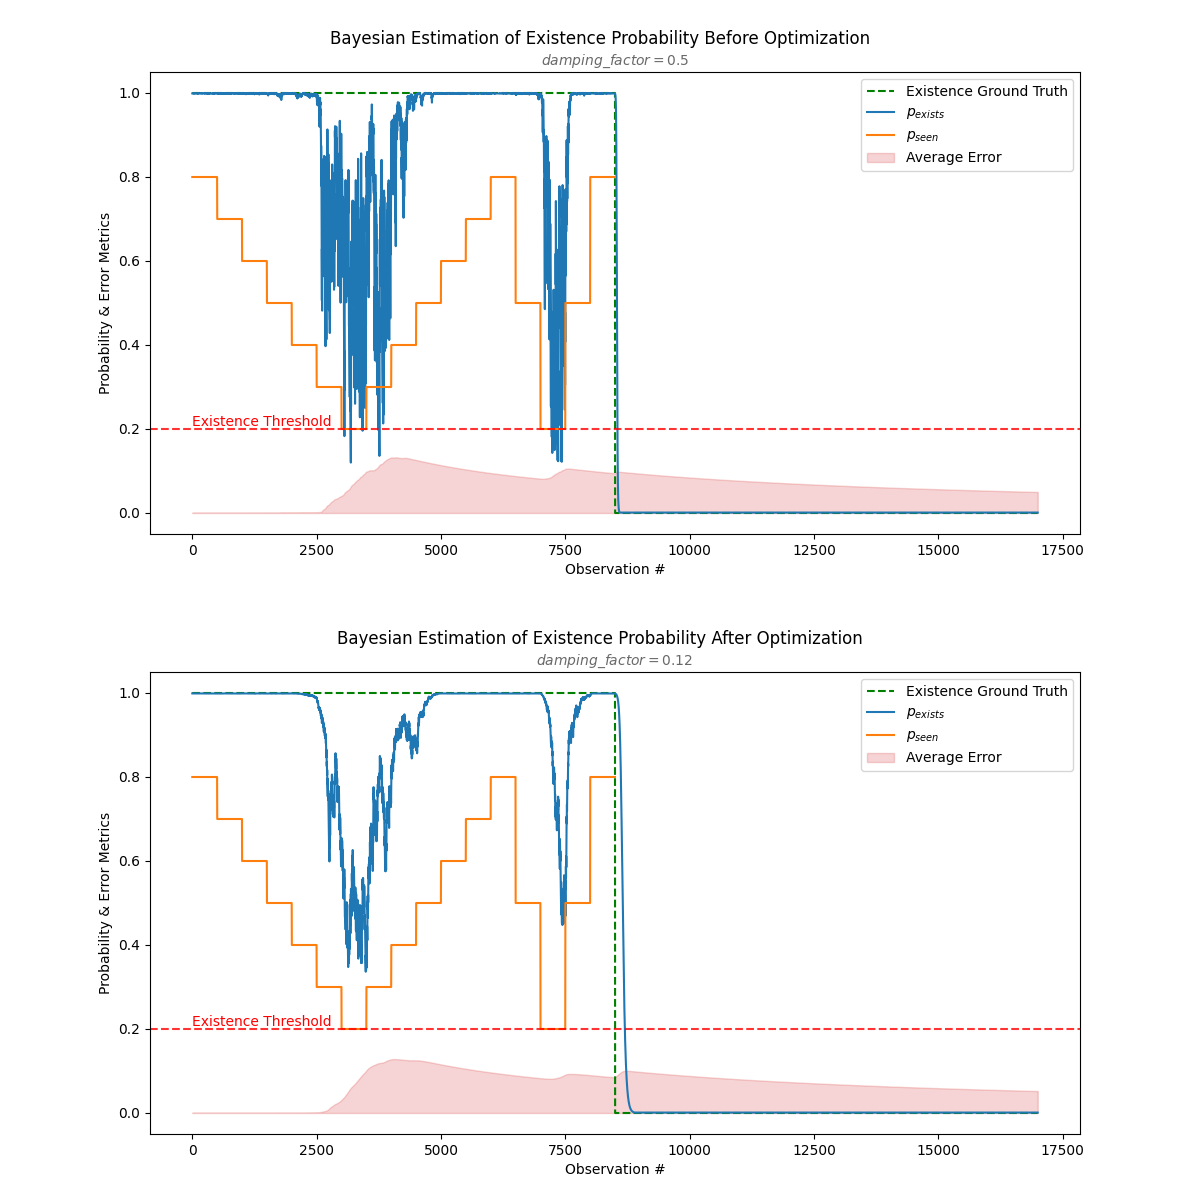
\includegraphics[width=0.8\textwidth]{resources/damping_coefficient_selection_results.png}
    \caption{Damping Coefficient Selection Results.}
    \label{fig:damping_coefficient_selection}
\end{figure}